\documentclass[10pt]{article}
\usepackage[polish]{babel}
\usepackage[utf8]{inputenc}
\usepackage[T1]{fontenc}
\usepackage{multirow}
\usepackage{amsmath}
\usepackage{amsfonts}
\usepackage{amssymb}
\usepackage[version=4]{mhchem}
\usepackage{stmaryrd}
\usepackage{graphicx}
\usepackage[export]{adjustbox}
\graphicspath{ {./images/} }

\title{EGZAMIN MATURALNY W ROKU SZKOLNYM 2018/2019 }

\author{MATEMATYKA\\
POZIOM PODSTAWOWY\\
FORMUŁA OD 2015\\
(„NOWA MATURA")}
\date{}


\newcommand\Varangle{\mathop{{<\!\!\!\!\!\text{\small)}}\:}\nolimits}

\begin{document}
\maketitle


\section*{ZASADY OCENIANIA ROZWIĄZAŃ ZADAŃ }
ARKUSZ MMA-P1

\section*{Zadania zamknięte}
Punkt przyznaje się za wskazanie poprawnej odpowiedzi.\\
Zadanie 1. (0-1)

\begin{center}
\begin{tabular}{|c|c|c|c|}
\hline
Wymagania ogólne & Wymagania szczególowe & \multicolumn{2}{|l|}{Poprawna odpowiedź} \\
\hline
\multirow[t]{2}{*}{II. Wykorzystanie i interpretowanie reprezentacji.} & \multirow[t]{2}{*}{1. Liczby rzeczywiste. Zdający wykorzystuje definicję logarytmu i stosuje w obliczeniach wzory na logarytm iloczynu, logarytm ilorazu i logarytm potęgi o wykładniku naturalnym (1.6).} & \begin{tabular}{l}
Wersja \\
I \\
\end{tabular} & Wersja II \\
\hline
 &  & A & D \\
\hline
\end{tabular}
\end{center}

Zadanie 2. (0-1)

\begin{center}
\begin{tabular}{|l|l|c|c|}
\hline
\multirow{2}{*}{\begin{tabular}{l}
II. Wykorzystanie \\
i interpretowanie \\
reprezentacji. \\
\end{tabular}} & \begin{tabular}{l}
1. Liczby rzeczywiste. Zdajaçy oblicza potęgi \\
o wykładnikach wymiernych i stosuje prawa \\
działań na potegach o wykładnikach \\
wymiernych (1.4). \\
\end{tabular} & \begin{tabular}{c}
Wersja \\
I \\
\end{tabular} & \begin{tabular}{c}
Wersja \\
II \\
\end{tabular} \\
\cline { 3 - 4 }
 & B & C &  \\
\hline
\end{tabular}
\end{center}

\section*{Zadanie 3. (0-1)}
\begin{center}
\begin{tabular}{|l|l|c|c|}
\hline
\begin{tabular}{l}
III. Modelowanie \\
matematyczne. \\
\end{tabular} & \begin{tabular}{l}
1. Liczby rzeczywiste. Zdający wykonuje \\
obliczenia procentowe, oblicza podatki, zysk \\
z lokat (1.9). \\
\end{tabular} & \begin{tabular}{c}
Wersja \\
I \\
\end{tabular} & \begin{tabular}{c}
Wersja \\
II \\
\end{tabular} \\
\cline { 3 - 4 }
 &  & B & A \\
\hline
\end{tabular}
\end{center}

\section*{Zadanie 4. (0-1)}
\begin{center}
\begin{tabular}{|l|l|c|c|}
\hline
\multirow{2}{*}{\begin{tabular}{l}
I. Wykorzystanie \\
i tworzenie informacji. \\
\end{tabular}} & \begin{tabular}{l}
3. Równania i nierówności. Zdający sprawdza, \\
czy dana liczba rzeczywista jest rozwiązaniem \\
równania lub nierówności (3.1). \\
\end{tabular} & \begin{tabular}{c}
Wersja \\
I \\
\end{tabular} & \begin{tabular}{c}
Wersja \\
II \\
\end{tabular} \\
\cline { 3 - 4 }
 &  & D & C \\
\hline
\end{tabular}
\end{center}

Zadanie 5. (0-1)

\begin{center}
\begin{tabular}{|l|l|c|c|}
\hline
\multirow{3}{*}{\begin{tabular}{l}
I. Wykorzystanie \\
i tworzenie informacji. \\
\end{tabular}} & \begin{tabular}{l}
3. Równania i nierówności. Zdający \\
wykorzystuje interpretacje geometryczną \\
układu równań pierwszego stopnia z dwiema \\
niewiadomymi (3.2). \\
\end{tabular} & \begin{tabular}{c}
Wersja \\
I \\
\end{tabular} & \begin{tabular}{c}
Wersja \\
II \\
\end{tabular} \\
\cline { 3 - 4 }
 & B & A &  \\
\hline
\end{tabular}
\end{center}

Zadanie 6. (0-1)

\begin{center}
\begin{tabular}{|l|l|c|c|}
\hline
\multirow{2}{*}{\begin{tabular}{l}
I. Wykorzystanie \\
i tworzenie informacji. \\
\end{tabular}} & \begin{tabular}{l}
3. Równania i nierówności. Zdający \\
rozwiązuje proste równania wymierne, \\
prowadzące do równań liniowych lub \\
kwadratowych (3.8). \\
\end{tabular} & \begin{tabular}{c}
Wersja \\
I \\
\end{tabular} & \begin{tabular}{c}
Wersja \\
II \\
\end{tabular} \\
\cline { 3 - 4 }
 & C & A &  \\
\hline
\end{tabular}
\end{center}

\section*{Zadanie 7. (0-1)}
\begin{center}
\begin{tabular}{|l|l|c|c|}
\hline
II. Wykorzystanie \\
i interpretowanie \\
reprezentacji. \\
\end{tabular}
\end{center} \begin{tabular}{l}
4. Funkcje. Zdający oblicza ze wzoru wartość \\
funkcji dla danego argumentu. Posługuje się \\
poznanymi metodami rozwiązywania równań \\
do obliczenia, dla jakiego argumentu funkcja \\
przyjmuje daną wartość (4.2). \\
\end{tabular} \begin{tabular}{c}
Wersja \\
I \\
\end{tabular} \begin{tabular}{c}
Wersja \\
II \\
\end{tabular}

Zadanie 8. (0-1)

\begin{center}
\begin{tabular}{|l|l|c|c|}
\hline
 & \begin{tabular}{l}
4. Funkcje. Zdajaccy odczytuje z wykresu \\
własności funkcji (dziedzine, zbiór wartości, \\
\end{tabular} & \begin{tabular}{c}
Wersja \\
II \\
\end{tabular} & \begin{tabular}{c}
Wersja \\
II \\
\end{tabular} \\
\cline { 3 - 4 }
\begin{tabular}{l}
i interpretowanie \\
reprezentacji. \\
\end{tabular} & \begin{tabular}{l}
miejsca zerowe, maksymalne przedziały, \\
w których funkcja maleje, rośnie, ma stały \\
znak; punkty, w których funkcja przyjmuje \\
w podanym przedziale wartość największą \\
lub najmniejszą) (4.3). \\
\end{tabular} & C & D \\
\hline
\end{tabular}
\end{center}

Zadanie 9. (0-1)

\begin{center}
\begin{tabular}{|l|l|c|c|}
\hline
 & \begin{tabular}{l}
4. Funkcje. Zdajaçy odczytuje z wykresu \\
własności funkcji (dziedzinę, zbiór wartości, \\
\end{tabular} & \begin{tabular}{c}
Wersja \\
II \\
\end{tabular} & \begin{tabular}{c}
Wersja \\
II \\
\end{tabular} \\
\cline { 3 - 4 }
\begin{tabular}{l}
i interpretowanie \\
reprezentacji. \\
\end{tabular} & \begin{tabular}{l}
miejsca zerowe, maksymalne przedziały, \\
w których funkcja maleje, rośnie, ma stały \\
znak; punkty, w których funkcja przyjmuje \\
w podanym przedziale wartość największą \\
lub najmniejszą) (4.3). \\
\end{tabular} & D & A \\
\hline
\end{tabular}
\end{center}

Zadanie 10. (0-1)

\begin{center}
\begin{tabular}{|l|l|c|c|}
\hline
II. Wykorzystanie &  &  &  \\
\begin{tabular}{l}
i interpretowanie \\
reprezentacji. \\
\end{tabular} & \begin{tabular}{l}
4. Funkcje. Zdajacy wykorzystuje własności \\
funkcji liniowej i kwadratowej do interpretacji \\
\end{tabular} & \begin{tabular}{c}
Wersja \\
Iagadnień geometrycznych, fizycznych itp. \\
\end{tabular} & \begin{tabular}{c}
Wersja \\
II \\
\end{tabular} \\
\cline{4-4}
 & \begin{tabular}{l}
Itakże osadzonych w kontekście praktycznym) \\
(4.12). \\
\end{tabular} & D & B \\
\hline
\end{tabular}
\end{center}

Zadanie 11. (0-1)

$\left.$\textbackslash begin\{tabular\}\{|l|l|c|c|\}\\
\textbackslash hline III. Modelowanie \\
\\
matematyczne.

 \begin{tabular}{l}
\end{tabular}

\begin{enumerate}
  \setcounter{enumi}{4}
  \item Ciągi. Zdający stosuje wzór na $n$-ty wyraz \\
\\
i na sumę $n$ początkowych wyrazów ciągu \\
\\
arytmetycznego (5.3).
\end{enumerate}

 \begin{tabular}{c}
\end{tabular}

Wersja \\
\\
I

 \begin{tabular}{c}
\end{tabular}

Wersja \\
\\
II

 \textbackslash right\textbackslash rvert, \begin{tabular}{c}
\end{tabular}

A \\
\\
\textbackslash cline \{ 3 - 4 \}\\
\textbackslash end\{tabular\}

Zadanie 12. (0-1)

$\left.$\textbackslash begin\{tabular\}\{|l|l|c|c|\}\\
\textbackslash hline III. Modelowanie \\
\\
matematyczne.

 \begin{tabular}{l}
\end{tabular}

\begin{enumerate}
  \setcounter{enumi}{4}
  \item Ciągi. Zdający stosuje wzór na $n$-ty wyraz \\
\\
i na sumę $n$ początkowych wyrazów ciągu \\
\\
geometrycznego (5.4).
\end{enumerate}

 \begin{tabular}{c}
\end{tabular}

Wersja \\
\\
I

 \begin{tabular}{c}
\end{tabular}

Wersja \\
\\
II

 \textbackslash right\textbackslash rvert, \begin{tabular}{c}
\end{tabular}

A \\
\\
\textbackslash cline \{ 3 - 4 \}\\
\textbackslash end\{tabular\}

\section*{Zadanie 13. (0-1)}
\begin{center}
\begin{tabular}{|l|l|c|c|}
\hline
\multirow{2}{*}{\begin{tabular}{l}
II. Wykorzystanie \\
i interpretowanie \\
reprezentacji. \\
\end{tabular}} & \begin{tabular}{l}
6. Trygonometria. Zdający znając wartość \\
jednej z funkcji: sinus lub cosinus, wyznacza \\
wartości pozostałych funkcji tego samego kąta \\
ostrego (6.5). \\
\end{tabular} & \begin{tabular}{c}
Wersja \\
I \\
\end{tabular} & \begin{tabular}{c}
Wersja \\
II \\
\end{tabular} \\
\cline{3-4}
 & D & A &  \\
\hline
\end{tabular}
\end{center}

\section*{Zadanie 14. (0-1)}
\begin{center}
\begin{tabular}{|l|l|c|c|}
\hline
\multirow{2}{*}{\begin{tabular}{l}
IV. Użycie i tworzenie \\
strategii. \\
\end{tabular}} & \begin{tabular}{l}
7. Planimetria. Zdający stosuje zależności \\
między kątem środkowym i kątem wpisanym \\
\end{tabular} & \begin{tabular}{c}
Wersja \\
I \\
\end{tabular} & \begin{tabular}{c}
Wersja \\
II \\
\end{tabular} \\
\cline { 3 - 4 }
 & A 1$).$ & D &  \\
\hline
\end{tabular}
\end{center}

Zadanie 15. (0-1)

\begin{center}
\begin{tabular}{|l|l|c|c|}
\hline
\multirow{2}{*}{\begin{tabular}{l}
I. Wykorzystanie \\
i tworzenie informacji. \\
\end{tabular}} & \begin{tabular}{l}
7. Planimetria. Zdający rozpoznaje trójkąty \\
podobne i wykorzystuje cechy podobieństwa \\
trójkątów (7.3). \\
\end{tabular} & \begin{tabular}{c}
Wersja \\
I \\
\end{tabular} & \begin{tabular}{c}
Wersja \\
II \\
\end{tabular} \\
\cline { 3 - 4 }
 & C & B &  \\
\hline
\end{tabular}
\end{center}

Zadanie 16. (0-1)\\
IV. Użycie i tworzenie strategii.\\
7. Planimetria. Zdający korzysta z własności funkcji trygonometrycznych w łatwych obliczeniach geometrycznych, w tym ze wzoru na pole trójkąta ostrokątnego o danych dwóch bokach i kącie między nimi (7.4).

\begin{center}
\begin{tabular}{|c|c|}
\hline
\begin{tabular}{c}
Wersja \\
I \\
\end{tabular} & \begin{tabular}{c}
Wersja \\
II \\
\end{tabular} \\
\hline
A & D \\
\hline
\end{tabular}
\end{center}

Zadanie 17. (0-1)

\begin{center}
\begin{tabular}{|l|l|c|c|}
\hline
\multirow{2}{*}{\begin{tabular}{l}
II. Wykorzystanie \\
i interpretowanie \\
reprezentacji. \\
\end{tabular}} & \begin{tabular}{l}
8. Geometria na płaszczyźnie kartezjańskiej. \\
Zdający bada równoległość i prostopadłość \\
\end{tabular} & \begin{tabular}{c}
Wersja \\
I \\
\end{tabular} & \begin{tabular}{c}
Wersja \\
II \\
krostych na podstawie ich równań \\
\end{tabular} \\
\cline{3-4}
 & D & B &  \\
\hline
\end{tabular}
\end{center}

Zadanie 18. (0-1)

\begin{center}
\begin{tabular}{|l|l|c|c|}
\hline
II. Wykorzystanie & \begin{tabular}{l}
8. Geometria na płaszczyźnie kartezjańskiej. \\
Zdający wyznacza równanie prostej, która jest \\
i interpretowanie \\
reprezentacji. \\
\end{tabular} & \begin{tabular}{l}
Wersja \\
Iówoległa lub prostopadła do prostej danej \\
\end{tabular} & \begin{tabular}{c}
Wersja \\
w postaci kierunkowej i przechodzi przez \\
dany punkt (8.3). \\
\end{tabular} \\
\cline{3-4}
 & B & C &  \\
\hline
\end{tabular}
\end{center}

Zadanie 19. (0-1)

\begin{center}
\begin{tabular}{|l|l|c|c|}
\hline
 & \begin{tabular}{l}
8. Geometria na płaszczyźnie kartezjańskiej. \\
Zdający znajduje obrazy niektórych figur \\
geometrycznych (punktu, prostej, odcinka, \\
II. Wykorzystanie \\
\end{tabular} & \begin{tabular}{c}
Wersja \\
I \\
\end{tabular} & \begin{tabular}{c}
Wersja \\
II \\
\end{tabular} \\
\cline{4-4}
\begin{tabular}{l}
i interpretowanie \\
reprezentacji. \\
\end{tabular} & \begin{tabular}{l}
lrójkąta itp.) w symetrii osiowej \\
względem osi układu współrzędnych \\
i symetrii środkowej względem początku \\
układu (8.7). \\
\end{tabular} & C & A \\
\hline
\end{tabular}
\end{center}

Zadanie 20. (0-1)

\begin{center}
\begin{tabular}{|l|l|c|c|}
\hline
\begin{tabular}{l}
II. Wykorzystanie \\
i interpretowanie \\
reprezentacji. \\
\end{tabular} & \begin{tabular}{l}
8. Geometria na płaszczyźnie kartezjańskiej. \\
Zdający oblicza odległość dwóch punktów (8.6). \\
\end{tabular} & \begin{tabular}{c}
Wersja \\
I \\
\end{tabular} & \begin{tabular}{c}
Wersja \\
II \\
\end{tabular} \\
\cline { 3 - 4 }
 & C & D &  \\
\hline
\end{tabular}
\end{center}

Zadanie 21. (0-1)

\begin{center}
\begin{tabular}{|l|l|c|c|}
\hline
\begin{tabular}{l}
II. Wykorzystanie \\
i interpretowanie \\
reprezentacji. \\
\end{tabular} & \begin{tabular}{l}
9. Stereometria. Zdający określa, jaką figurą \\
jest dany przekrój prostopadłościanu \\
płaszczyzną (9.5). \\
\end{tabular} & \begin{tabular}{c}
Wersja \\
I \\
\end{tabular} & \begin{tabular}{c}
Wersja \\
II \\
\end{tabular} \\
\cline { 2 - 4 }
 & \begin{tabular}{l}
G10. Figury płaskie. Zdający stosuje \\
twierdzenie Pitagorasa (G10.7). \\
\end{tabular} & B & D \\
\hline
\end{tabular}
\end{center}

Zadanie 22. (0-1)

\begin{center}
\begin{tabular}{|l|l|c|c|}
\hline
\multirow{2}{|l|}{\begin{tabular}{l}
II. Wykorzystanie \\
i interpretowanie \\
reprezentacji. \\
\end{tabular}} & \begin{tabular}{l}
G11. Bryły. Zdający oblicza pole powierzchni \\
i objętość walca, stożka, kuli (G11.2). \\
\end{tabular} & \begin{tabular}{c}
Wersja \\
I \\
\end{tabular} & \begin{tabular}{c}
Wersja \\
II \\
\end{tabular} \\
\cline { 3 - 4 }
 &  & D & C \\
\hline
\end{tabular}
\end{center}

Zadanie 23. (0-1)

\begin{center}
\begin{tabular}{|l|l|c|c|}
\hline
\multirow{2}{*}{\begin{tabular}{l}
II. Wykorzystanie \\
i interpretowanie \\
reprezentacji. \\
\end{tabular}} & \begin{tabular}{l}
G9. Statystyka opisowa i wprowadzenie do \\
rachunku prawdopodobieństwa. Zdajajcy \\
wyznacza średnią arytmetyczną i medianę \\
zestawu danych (G9.4). \\
\end{tabular} & \begin{tabular}{c}
Wersja \\
I \\
\end{tabular} & \begin{tabular}{c}
Wersja \\
II \\
\end{tabular} \\
\cline{3-4}
 & B & C &  \\
\hline
\end{tabular}
\end{center}

Zadanie 24. (0-1)

\begin{center}
\begin{tabular}{|l|l|c|c|}
\hline
 & \begin{tabular}{l}
10. Elementy statystyki opisowej. Teoria \\
prawdopodobieństwa i kombinatoryka. \\
\end{tabular} & \begin{tabular}{c}
Wersja \\
I \\
\end{tabular} & \begin{tabular}{c}
Wersja \\
II \\
\end{tabular} \\
\cline { 3 - 4 }
\begin{tabular}{l}
III. Modelowanie \\
matematyczne. \\
\end{tabular} & \begin{tabular}{l}
Zdający zlicza obiekty w prostych sytuacjach \\
kombinatorycznych, niewymagających użycia \\
wzorów kombinatorycznych, stosuje regułę \\
mnożenia i regułę dodawania (10.2). \\
\end{tabular} & C & D \\
\hline
\end{tabular}
\end{center}

Zadanie 25. (0-1)

\begin{center}
\begin{tabular}{|l|l|c|c|}
\hline
 & \begin{tabular}{l}
10. Elementy statystyki opisowej. Teoria \\
III. Modelowanie \\
matematyczne. \\
\end{tabular} & \begin{tabular}{l}
2rawdopodobieństwa i kombinatoryka. \\
Zdajacy oblicza prawdopodobienstwa \\
w prostych sytuacjach, stosując klasyczną \\
definicję prawdopodobieństwa (10.3). \\
\end{tabular} & \begin{tabular}{c}
Wersja \\
I \\
\end{tabular} \\
\cline { 3 - 4 }
 & Wersja & II &  \\
\hline
\end{tabular}
\end{center}

\section*{Zadania otwarte}
Uwaga: Akceptowane sq wszystkie odpowiedzi merytorycznie poprawne i spetniajace warunki zadania.

\section*{Zadanie 26. (0-2)}
\begin{center}
\begin{tabular}{|l|l}
\hline
\begin{tabular}{l}
I. Wykorzystanie \\
i tworzenie informacji. \\
\end{tabular} & \begin{tabular}{l}
3. Równania i nierówności. Zdający korzysta z własności \\
iloczynu przy rozwiązywaniu równań typu $x(x+1)(x-7)=0$ \\
(3.7). \\
\end{tabular} \\
\hline
\end{tabular}
\end{center}

\section*{Schemat punktowania}
\section*{Zdający otrzymuje}
gdy wyznaczy wszystkie rozwiązania równania: $x=2, x=-1$ oraz $x=5$, o ile nie zastosuje niepoprawnej metody.

\section*{Zdający otrzymuje \\
 1 p. \\
 gdy:}
\begin{itemize}
  \item zapisze dwa równania $x^{3}-8=0$ i $x^{2}-4 x-5=0$ lub z zapisu wynika, że rozwiązuje te równania\\
albo
  \item wyznaczy poprawnie lub poda rozwiązania jednego z równań: $x^{3}-8=0$ lub $x^{2}-4 x-5=0$\\
i na tym zakończy lub dalej popełni błędy.
\end{itemize}

\section*{Uwagi}
\begin{enumerate}
  \item Jeżeli zdający jedynie poda wszystkie rozwiązania równania, bez zapisanych rachunków lub uzasadnienia, to otrzymuje 2 punkty.
  \item Jeżeli zdający poprawnie zapisze lewą stronę równania w postaci sumy jednomianów, znajdzie trzy rozwiązania: $-1,2,5$, ale nie uzasadni, że są to jedyne rozwiązania, to otrzymuje 1 punkt.
  \item Jeżeli na etapie przyrównywania czynników do zera jedynym błędem zdającego jest błąd przy rozkładzie wielomianu $x^{3}-8$, to zdający może otrzymać $\mathbf{1}$ punkt za całe rozwiązanie.
\end{enumerate}

\section*{Przykładowe rozwiązanie}
Iloczyn $\left(x^{3}-8\right)\left(x^{2}-4 x-5\right)=0$ jest równy 0 , jeśli przynajmniej jeden z czynników jest równy 0 .\\
Zatem $x^{3}-8=0$ lub $x^{2}-4 x-5=0$.\\
Równanie $x^{3}-8=0$ ma jedno rozwiązanie $x=2$.\\
Równanie $x^{2}-4 x-5=0$ doprowadzamy do postaci iloczynowej $(x+1) \cdot(x-5)=0$.\\
Przynajmniej jeden z czynników $(x+1)$ lub $(x-5)$ jest równy 0 , czyli $x=-1$ lub $x=5$.\\
Zatem rozwiązaniami równania $\left(x^{3}-8\right)\left(x^{2}-4 x-5\right)=0$ są liczby: $x=2, x=-1$ oraz $x=5$.

\section*{Zadanie 27. (0-2)}
II. Wykorzystanie i interpretowanie reprezentacji.\\
3. Równania i nierówności. Zdający rozwiązuje nierówności kwadratowe z jedną niewiadomą (3.5).

\section*{Schemat punktowania}
Zdający otrzymuje\\
gdy:

\begin{itemize}
  \item poda zbiór rozwiązań nierówności: $\left(-\infty, \frac{4}{3}\right) \cup(4,+\infty)$ lub $x \in\left(-\infty, \frac{4}{3}\right) \cup(4,+\infty)$, lub $x<\frac{4}{3} \vee x>4$\\
albo
  \item poda zbiór rozwiązań nierówności w postaci graficznej z poprawnie zaznaczonymi końcami przedziałów\\
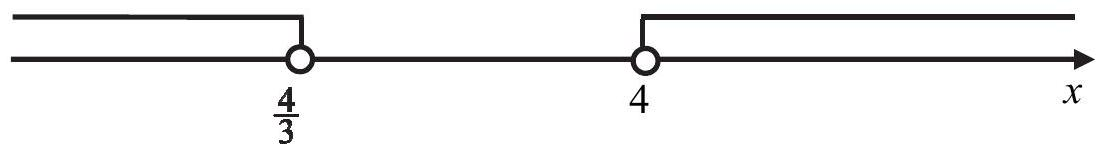
\includegraphics[max width=\textwidth, center]{2025_02_07_cbaae63d39acb23a5920g-08}
\end{itemize}

Zdający otrzymuje 1 p.\\
gdy:

\begin{itemize}
  \item zrealizuje pierwszy etap rozwiązania i na tym zakończy lub błędnie zapisze zbiór rozwiązań nierówności, np.
  \item obliczy lub poda pierwiastki trójmianu kwadratowego $x_{1}=\frac{4}{3}$ oraz $x_{2}=4$ i na tym zakończy lub błędnie zapisze zbiór rozwiązań nierówności;
  \item zaznaczy na wykresie miejsca zerowe funkcji $f$ określonej wzorem $f(x)=3 x^{2}-16 x+16$ i na tym zakończy lub błędnie zapisze zbiór rozwiązań nierówności
  \item popełni błędy przy wyznaczaniu pierwiastków trójmianu kwadratowego $3 x^{2}-16 x+16$, ale otrzyma dwa różne pierwiastki trójmianu kwadratowego i konsekwentnie do popełnionych błędów wyznaczy zbiór rozwiązań nierówności.
\end{itemize}

\section*{Uwagi}
\begin{enumerate}
  \item Jeżeli zdający wyznacza pierwiastki trójmianu kwadratowego w przypadku, gdy obliczony wyróżnik $\Delta$ jest ujemny, to otrzymuje $\mathbf{0}$ punktów za całe rozwiązanie.
  \item Jeżeli zdający podaje pierwiastki bez związku z trójmianem kwadratowym z zadania, to oznacza, że nie podjął realizacji 1. etapu rozwiązania i w konsekwencji otrzymuje 0 punktów za całe rozwiązanie.
  \item Akceptujemy zapisanie odpowiedzi w postaci: $x<\frac{4}{3}$ i $x>4, x<\frac{4}{3}$ oraz $x>4$, itp.
  \item Jeżeli zdający poprawnie obliczy pierwiastki trójmianu $x_{1}=\frac{4}{3}, x_{2}=4$ i błędnie zapisze odpowiedź, np. $x \in\left(-\infty,-\frac{4}{3}\right) \cup(4,+\infty)$, popełniając tym samym błąd przy przepisywaniu jednego z pierwiastków, to otrzymuje 2 punkty.
\end{enumerate}

\section*{Kryteria uwzględniające specyficzne trudności w uczeniu się matematyki}
Jeśli zdający pomyli porządek liczb na osi liczbowej, np. zapisze zbiór rozwiązań nierówności w postaci $(-\infty, 4) \cup\left(\frac{4}{3},+\infty\right),(+\infty, 4) \cup\left(\frac{4}{3},-\infty\right)$, to przyznajemy 2 punkty.

\section*{Przykładowe rozwiązanie}
Rozwiązanie nierówności kwadratowej składa się z dwóch etapów.\\
Pierwszy etap to wyznaczenie pierwiastków trójmianu kwadratowego: $3 x^{2}-16 x+16$.\\
Drugi etap to zapisanie zbioru rozwiązań nierówności kwadratowej: $3 x^{2}-16 x+16>0$.\\
Pierwszy etap rozwiązania może zostać zrealizowany następująco:

\begin{itemize}
  \item obliczamy pierwiastki trójmianu kwadratowego $3 x^{2}-16 x+16$
  \item obliczamy wyróżnik tego trójmianu:
\end{itemize}

$$
\Delta=16 \cdot 16-4 \cdot 3 \cdot 16=4 \cdot 16=2^{2} \cdot 4^{2} \text { i stąd } x_{1}=\frac{16-8}{6}=\frac{4}{3} \text { oraz } x_{2}=\frac{16+8}{6}=4
$$

albo

\begin{itemize}
  \item stosujemy wzory Viète'a:
\end{itemize}

$$
x_{1} \cdot x_{2}=\frac{16}{3} \text { oraz } x_{1}+x_{2}=\frac{16}{3}, \text { stąd } x_{1}=\frac{4}{3} \text { oraz } x_{2}=4 .
$$

Drugi etap rozwiązania.\\
Podajemy zbiór rozwiązań nierówności: $\left(-\infty, \frac{4}{3}\right) \cup(4,+\infty)$ lub $x \in\left(-\infty, \frac{4}{3}\right) \cup(4,+\infty)$.

Zadanie 28. (0-2)

\begin{center}
\begin{tabular}{|l|l|}
\hline
V. Rozumowanie & 2. Wyrażenia algebraiczne. Zdający używa wzorów skróconego \\
i argumentacja. & mnożenia na $(a \pm b)^{2}$ oraz $a^{2}-b^{2}(2.1)$. \\
\end{tabular}
\end{center}

\section*{Schemat punktowania}
\section*{Zdający otrzymuje 2 p. \\
 gdy przeprowadzi pełne rozumowanie.}
Zdający otrzymuje ........................................................................................................... 1 p.\\
gdy

\begin{itemize}
  \item zapisze nierówność w postaci, zawierającej po jednej stronie 0, a po drugiej sumę wyrażeń algebraicznych, będących wielokrotnościami kwadratów liczb lub stanowiących jedną stronę wzoru skróconego mnożenia, którego druga strona jest kwadratem, np.:
\end{itemize}

$$
2 a^{2}+a^{2}-2 a b+b^{2}+2 b^{2} \geq 0
$$

albo

\begin{itemize}
  \item zapisze oszacowanie $3 a^{2}-2 a b+3 b^{2} \geq a^{2}-2 a b+b^{2}$,\\
albo
  \item obliczy wyróżnik trójmianu kwadratowego w zależności od zmiennej a lub $b$, występującego po jednej stronie nierówności, gdy po drugiej stronie jest 0 , i stwierdzi, że jest on niedodatni,\\
albo
  \item rozważa dwa przypadki: w pierwszym stwierdza, że gdy $a b \leq 0$, to nierówność jest prawdziwa, a drugim doprowadza nierówność do postaci $\frac{a}{b}+\frac{b}{a} \geq \frac{2}{3}$,\\
albo
  \item rozważa dwa przypadki: w jednym dzieli stronami nierówność przez $b^{2}$ lub przez $a^{2}$, a w drugim przyjmuje, że $a$ lub $b$ jest równe 0 , oraz w przypadku, w którym dzieli stronami nierówność i obliczy wyróżnik otrzymanego trójmianu kwadratowego,\\
albo
  \item zapisze, że prawdziwa jest nierówność $2 a^{2}+2 b^{2} \geq 0$ oraz zapisze, że prawdziwa jest nierówność $(a-b)^{2} \geq 0$ i przedstawi tę nierówność w postaci równoważnej $a^{2}-2 a b+b^{2} \geq 0$,\\
albo
  \item wskaże, że przeprowadza dowód nie wprost, zapisze nierówność $3 a^{2}-2 a b+3 b^{2}<0$ oraz zapisze jeden z dwóch poniższych komentarzy:
  \item nierówność $(a-b)^{2}<0$ jest nieprawdziwa;
  \item nierówność $(a-b)^{2} \geq 0$ jest prawdziwa oraz nierówność $2 a^{2}+2 b^{2}<0$ jest nieprawdziwa\\
i na tym zakończy lub dalej popełnia błędy.
\end{itemize}

\section*{Uwagi}
\begin{enumerate}
  \item Jeżeli zdający sprawdza prawdziwość nierówności jedynie dla wybranych wartości $a$ i $b$, to otrzymuje $\mathbf{0}$ punktów za całe rozwiązanie.
  \item Jeżeli zdający zakończy rozumowanie, zapisując nierówność $2 a^{2}+(a-b)^{2}+2 b^{2} \geq 0$ lub $\left(a-\frac{1}{3} b\right)^{2}+\frac{8}{9} b^{2} \geq 0$ i nie przedstawi komentarza uzasadniającego przyjmowanie wyłącznie nieujemnych wartości przez wyrażenie zapisane po lewej stronie nierówności, to otrzymuje 1 punkt.
  \item Jeżeli zdający w IV sposobie rozwiązania pominie przypadek $b=0$ lub $a=0$, to za całe rozwiązanie może otrzymać co najwyżej 1 punkt.
  \item Jeżeli zdający w V sposobie rozwiązania pominie przypadek $a b \leq 0$, to za całe rozwiązanie może otrzymać co najwyżej $\mathbf{1}$ punkt, o ile wykaże prawdziwość nierówności w przypadku $a b>0$.
  \item Jeżeli zdający po uzasadnieniu prawdziwości nierówności $a^{2}-2 a b+b^{2} \geq 0$ zapisze nierówność $3 a^{2}-2 a b+3 b^{2} \geq 0$ i na tym zakończy, to za całe rozwiązanie otrzymuje 1 punkt.
\end{enumerate}

\section*{Przykładowe rozwiązania}
\section*{I sposób}
Przekształcamy równoważnie nierówność i otrzymujemy kolejno:

$$
\begin{gathered}
3 a^{2}-2 a b+3 b^{2} \geq 0, \\
2 a^{2}+a^{2}-2 a b+b^{2}+2 b^{2} \geq 0, \\
2 a^{2}+(a-b)^{2}+2 b^{2} \geq 0
\end{gathered}
$$

Lewa strona nierówności jest sumą trzech liczb nieujemnych: $2 a^{2}-$ jako wielokrotność kwadratu liczby, $(a-b)^{2}$ - jako kwadrat liczby, $2 b^{2}$ - jako wielokrotność kwadratu liczby.

Zatem z lewej strony nierówności występuje wyrażenie przyjmujące wartość nieujemną, czyli nierówność jest prawdziwa dla dowolnych rzeczywistych liczb $a$ i $b$.

To kończy dowód.

\section*{Uwaga}
Całe rozumowanie można zapisać w postaci

$$
3 a^{2}-2 a b+3 b^{2} \geq a^{2}-2 a b+b^{2}=(a-b)^{2} \geq 0
$$

co jest prawdą dla dowolnych liczb rzeczywistych $a, b$.

\section*{II sposób}
Przekształcamy równoważnie nierówność i otrzymujemy kolejno:

$$
\begin{gathered}
3 a^{2}-2 a b+3 b^{2} \geq 0 \\
a^{2}-\frac{2}{3} a b+b^{2} \geq 0 \\
\left(a-\frac{1}{3} b\right)^{2}-\frac{1}{9} b^{2}+b^{2} \geq 0 \\
\left(a-\frac{1}{3} b\right)^{2}+\frac{8}{9} b^{2} \geq 0
\end{gathered}
$$

Lewa strona nierówności jest sumą dwóch liczb nieujemnych: $\left(a-\frac{1}{3} b\right)^{2}-$ jako kwadrat liczby, $\frac{8}{9} b^{2}-$ jako wielokrotność kwadratu liczby.

Zatem z lewej strony nierówności występuje wyrażenie przyjmujące wartość nieujemną, czyli nierówność jest prawdziwa dla dowolnych rzeczywistych liczb $a$ i $b$.

To kończy dowód.

\section*{III sposób}
Wyrażenie z lewej strony jest trójmianem kwadratowym dla zmiennej $a$, z parametrem $b$. Obliczamy wyróżnik tego trójmianu kwadratowego:

$$
\Delta=(-2 b)^{2}-4 \cdot 3 \cdot 3 b^{2}=4 b^{2}-36 b^{2}=-32 b^{2} .
$$

Obliczony wyróżnik trójmianu kwadratowego jest niedodatni dla dowolnej liczby rzeczywistej $b$. Zatem trójmian kwadratowy nie ma pierwiastków lub ma jeden pierwiastek rzeczywisty. Przy najwyższej potędze trójmianu kwadratowego stoi liczba dodatnia 3, zatem lewa strona nierówności przyjmuje wartości nieujemne dla dowolnej zmiennej rzeczywistej $a$. Oznacza to, że nierówność jest prawdziwa dla dowolnych rzeczywistych liczb $a$ i $b$.

To kończy dowód.

\section*{IV sposób}
Rozważmy dwa przypadki.

\begin{enumerate}
  \item $b=0$
  \item $b \neq 0$
\end{enumerate}

W pierwszym przypadku otrzymujemy nierówność $3 a^{2} \geq 0$, która jest prawdziwa dla dowolnej liczby rzeczywistej $a$, bo wyrażenie po lewej stronie jest wielokrotnością kwadratu liczby. Zatem nierówność $3 a^{2}-2 a b+3 b^{2} \geq 0$ jest prawdziwa w przypadku, gdy $b=0$.

W drugim przypadku możemy podzielić obie strony nierówności $3 a^{2}-2 a b+3 b^{2} \geq 0$ przez $b^{2}$. Otrzymujemy nierówność: $3\left(\frac{a}{b}\right)^{2}-2 \frac{a}{b}+3 \geq 0$.

Obliczamy wyróżnik trójmianu kwadratowego zmiennej $x$, gdzie $x=\frac{a}{b}$, występującego z lewej strony nierówności:

$$
\Delta=(-2)^{2}-4 \cdot 3 \cdot 3=4-36=-32 .
$$

Obliczony wyróżnik trójmianu kwadratowego jest ujemny, zatem trójmian kwadratowy nie ma pierwiastków rzeczywistych. Przy najwyższej potędze trójmianu kwadratowego stoi liczba dodatnia 3, zatem lewa strona nierówności przyjmuje zawsze wartość dodatnią. Oznacza to, że nierówność jest prawdziwa dla dowolnej liczby $a$ i dowolnej liczby $b$ różnej od zera.

Z rozważonych dwóch przypadków wynika, że nierówność jest prawdziwa dla dowolnych rzeczywistych liczb $a$ i $b$.

To kończy dowód.\\
V sposób (przypadki ze względu na znak $a b$ ).\\
Rozważmy dwa przypadki.

\begin{enumerate}
  \item Gdy $a b \leq 0$. Wtedy nierówność $3 a^{2}-2 a b+3 b^{2} \geq 0$ jest prawdziwa, gdyż po jej lewej stronie jest suma trzech nieujemnych składników $3 a^{2},-2 a b, 3 b^{2}$.
  \item Gdy $a b>0$. Wtedy nierówność zapisujemy w postaci równoważnej $3 a^{2}+3 b^{2} \geq 2 a b$. Obie strony tej nierówności możemy wtedy podzielić przez dodatnią liczbę $3 a b$, otrzymując nierówność
\end{enumerate}

$$
\frac{a}{b}+\frac{b}{a} \geq \frac{2}{3} .
$$

Z twierdzenia o sumie liczby dodatniej i jej odwrotności wynika, że $\frac{a}{b}+\frac{b}{a} \geq 2>\frac{2}{3}$.\\
To kończy dowód.\\
VI sposób (dowód nie wprost)\\
Załóżmy, nie wprost, że dla pewnych liczb rzeczywistych $a$ i $b$ prawdziwa jest nierówność

$$
3 a^{2}-2 a b+3 b^{2}<0 .
$$

Ponieważ $2 a^{2}+2 b^{2} \geq 0$, więc nierówność ta byłaby prawdziwa tylko wtedy, gdyby $a^{2}-2 a b+b^{2}<0$, czyli $(a-b)^{2}<0$, co jest nieprawdą.

Otrzymana sprzeczność oznacza, że nierówność $3 a^{2}-2 a b+3 b^{2}<0$ jest fałszywa.\\
Prawdziwa zatem jest nierówność: $3 a^{2}-2 a b+3 b^{2} \geq 0$

To kończy dowód.

VII sposób\\
Dla dowolnych liczb rzeczywistych $a, b$ prawdziwe są nierówności

$$
(a-b)^{2} \geq 0 \text { oraz } 2 a^{2}+2 b^{2} \geq 0
$$

czyli

$$
a^{2}-2 a b+b^{2} \geq 0 \text { oraz } 2 a^{2}+2 b^{2} \geq 0
$$

Dodając te nierówności stronami, co możemy zrobić, gdyż nierówności są tak samo skierowane, otrzymujemy

$$
a^{2}-2 a b+b^{2}+2 a^{2}+2 b^{2} \geq 0,
$$

czyli

$$
3 a^{2}-2 a b+3 b^{2} \geq 0
$$

To kończy dowód.

Zadanie 29. (0-2)\\
V. Rozumowanie i argumentacja.

\section*{Schemat punktowania}
\section*{Zdający otrzymuje \\
 2 p. \\
 gdy przeprowadzi pełne rozumowanie.}
\section*{Zdający otrzymuje}
 1 p. gdy wykorzysta równość kątów przy podstawie w trójkątach równoramiennych $B C S$ i $A B S$ oraz\begin{itemize}
  \item zapisze zależność między kątami $\alpha$ i $A B S$, np.: $|\Varangle A B S|=|\Varangle B A S|=2 \alpha$\\
albo
  \item zapisze zależność między kątami $\alpha, D S A$ oraz dowolnym kątem trójkąta $A B S$ w postaci układu dwóch równań z trzema niewiadomymi, np.: $\alpha+\gamma+\beta=180^{\circ}$ i $\beta=180^{\circ}-4 \alpha$\\
i na tym zakończy lub dalej popełni błędy.
\end{itemize}

\section*{Uwagi}
\begin{enumerate}
  \item Rozwiązanie uznajemy za pełne, jeżeli z zapisów zdającego wynikają kolejne kroki rozumowania.
  \item Jeżeli zdający zaznaczy na rysunku zależności między kątami, ale nie opatrzy rozwiązania stosownym wyjaśnieniem, to może otrzymać co najwyżej 1 punkt. Tego typu sytuacje ilustrują poniższe rysunki.\\
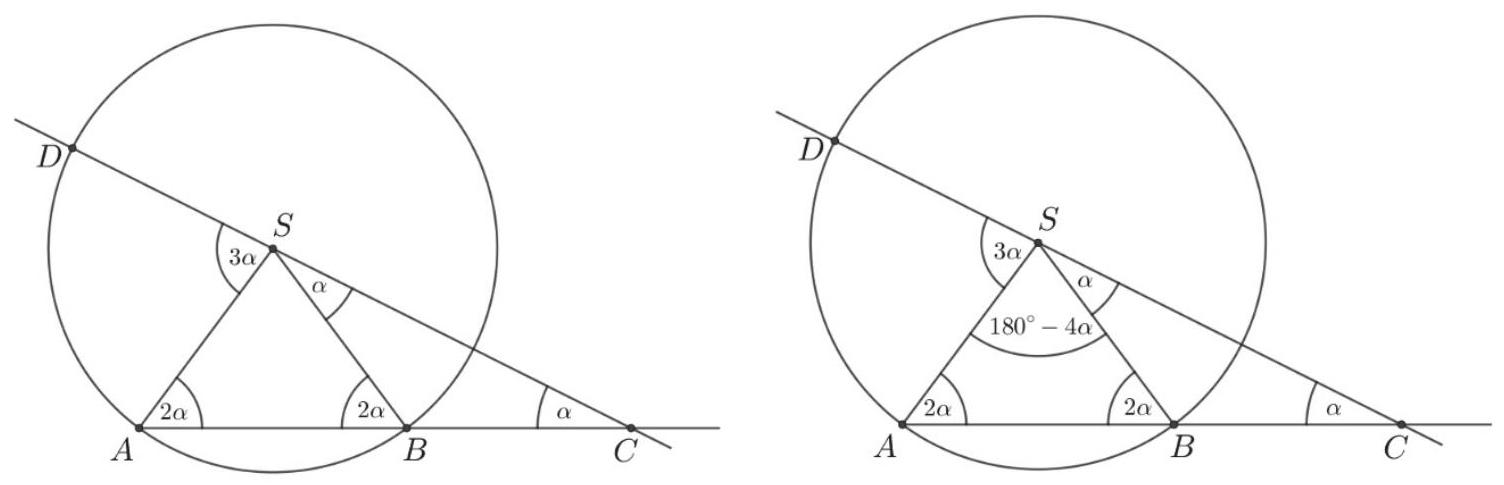
\includegraphics[max width=\textwidth, center]{2025_02_07_cbaae63d39acb23a5920g-15}
  \item Jeżeli zdający zaznaczy na rysunku kąty trójkątów $B C S, A B S$ i kąt $A S D$ i na tym poprzestanie, to otrzymuje $\mathbf{0}$ punktów. Tę sytuację ilustruje poniższy rysunek.\\
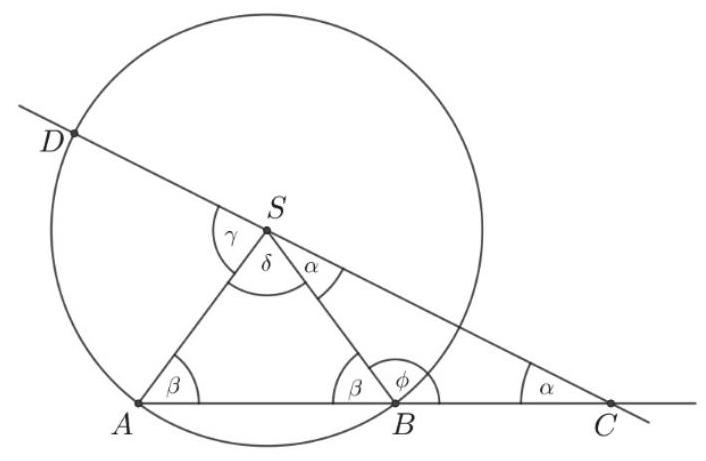
\includegraphics[max width=\textwidth, center]{2025_02_07_cbaae63d39acb23a5920g-16}
  \item Jeżeli zdający przyjmuje konkretne miary kątów, to otrzymuje $\mathbf{0}$ punktów.
\end{enumerate}

\section*{Przykładowe rozwiązanie}
Z założenia trójkąt $C S B$ jest równoramienny i $|B S|=|B C|$, więc $|\Varangle B S C|=|\Varangle B C S|$. Zatem $|\Varangle B C S|=|\Varangle A C S|=\alpha$. Wynika stąd, że $|\Varangle C B S|=180^{\circ}-2 \alpha$, a więc $|\Varangle A B S|=2 \alpha$. Ponieważ trójkąt $A B S$ jest równoramienny i $|A S|=|B S|$, więc $|\Varangle B A S|=2 \alpha$.\\
Zatem $|\Varangle A S B|=180^{\circ}-4 \alpha$.\\
Zauważmy, że

$$
|\Varangle A S D|+|\Varangle A S B|+|\Varangle B S C|=180^{\circ}
$$

Otrzymujemy zatem równanie

$$
|\Varangle A S D|+180^{\circ}-4 \alpha+\alpha=180^{\circ},
$$

skąd wynika, że

$$
|\Varangle A S D|=3 \alpha .
$$

To kończy dowód.

Zadanie 30. (0-2)

\begin{center}
\begin{tabular}{|l|l|}
\hline
\begin{tabular}{l}
III. Modelowanie \\
matematyczne. \\
\end{tabular} & \begin{tabular}{l}
10. Elementy statystyki opisowej. Teoria prawdopodobieństwa \\
i kombinatoryka. Zdający oblicza prawdopodobieństwa \\
w prostych sytuacjach, stosując klasyczną definicję \\
prawdopodobieństwa (10.3). \\
\end{tabular} \\
\hline
\end{tabular}
\end{center}

\section*{Schemat punktowania}
\section*{Zdający otrzymuje \\
 gdy obliczy prawdopodobieństwo zdarzenia $A: P(A)=\frac{9}{25}$.}
Zdający otrzymuje $\qquad$ 1 p. gdy

\begin{itemize}
  \item obliczy liczbę wszystkich możliwych zdarzeń elementarnych: $|\Omega|=5^{2}=25$\\
albo
  \item obliczy (zaznaczy poprawnie w tabeli) liczbę zdarzeń elementarnych sprzyjających zdarzeniu $A:|A|=9$ i nie wskazuje przy tym niepoprawnych zdarzeń elementarnych sprzyjających zdarzeniu $A$,\\
albo
  \item zapisze przy stosowaniu drzewa probabilistycznego na dwóch etapach prawdopodobieństwa potrzebne do wyznaczenia końcowego wyniku oraz wskaże wszystkie sytuacje sprzyjające rozważanemu zdarzeniu,\\
albo
  \item wypisze wszystkie zdarzenia elementarne sprzyjające zdarzeniu $A$ lub wypisze wszystkie zdarzenia elementarne\\
i na tym zakończy lub dalej popełni błędy.
\end{itemize}

\section*{Uwagi}
\begin{enumerate}
  \item Jeżeli zdający popełni błąd przy wypisywaniu par i wypisze o jedną za mało lub o jedną za dużo, ale nie wypisze żadnej niewłaściwej i konsekwentnie do popełnionego błędu obliczy prawdopodobieństwo, to otrzymuje 1 punkt.
  \item Jeśli zdający rozwiąże zadanie do końca i otrzyma $P(A)>1$ lub $P(A)<0$, to otrzymuje za całe rozwiązanie 0 punktów, o ile końcowy wynik nie jest skutkiem błędu w działaniach na ułamkach.
  \item Jeżeli zdający stosuje drzewo probabilistyczne, w którym przynajmniej pięć gałęzi odpowiada sytuacjom sprzyjającym rozważanemu zdarzeniu, i zdający pominie jedną z takich gałęzi, to może otrzymać $\mathbf{1}$ punkt, jeśli doprowadzi rozumowanie do końca.
  \item Jeżeli zdający zapisze tylko: $P(A)=\frac{9}{25}$, to otrzymuje $\mathbf{1}$ punkt.
  \item Jeżeli zdający zapisze tylko: $|A|=9,|\Omega|=25, P(A)=\frac{9}{25}$, to otrzymuje $\mathbf{2}$ punkty.
  \item Jeżeli zdający zapisze prawdopodobieństwo $P(A)=\frac{3}{5} \cdot \frac{3}{5}$, to otrzymuje $\mathbf{2}$ punkty.
\end{enumerate}

\section*{Przykładowe rozwiązania}
\section*{I sposób (klasyczna definicja prawdopodobieństwa)}
Zdarzeniami elementarnymi w przestrzeni $\Omega$ są wszystkie pary liczb $(a, b)$, gdzie $a, b \in\{1,2,3,4,5\}$.\\
Jest to model klasyczny. Liczba wszystkich zdarzeń elementarnych jest równa $|\Omega|=5 \cdot 5=25$. Obliczamy liczbę zdarzeń elementarnych sprzyjających zdarzeniu $A$ polegającym na otrzymaniu liczb, których iloczyn jest liczbą nieparzystą, np. wypisując je i zliczając:\\
$A=\{(1,1),(1,3),(1,5),(3,1),(3,3),(3,5),(5,1),(5,3),(5,5)\}$.\\
Liczba zdarzeń elementarnych sprzyjających zdarzeniu $A$ jest więc równa 9 .\\
Prawdopodobieństwo zdarzenia $A$ jest równe: $P(A)=\frac{9}{25}$.

II sposób (metoda tabeli)

\begin{center}
\begin{tabular}{|c|c|c|c|c|c|c|c|c|c|c|}
\hline
$(1,1)$ & $(1,2)$ & $(1,3)$ & $(1,4)$ & $(1,5)$ & \multicolumn{6}{|l|}{przedstawić w postaci kwadratowej tablicy} \\
\hline
$(2,1)$ & $(2,2)$ & $(2,3)$ & $(2,4)$ & $(2,5)$ & \multirow[b]{2}{*}{albo} &  &  &  &  &  \\
\hline
$(3,1)$ & $(3,2)$ & $(3,3)$ & $(3,4)$ & $(3,5)$ &  &  &  &  &  &  \\
\hline
$(4,1)$ & $(4,2)$ & $(4,3)$ & $(4,4)$ & $(4,5)$ & 1 & X & 2 & X & 4 & X \\
\hline
$(5,1)$ & $(5,2)$ & $(5,3)$ & $(5,4)$ & $(5,5)$ & 2 &  &  &  &  &  \\
\hline
 &  &  &  &  & 3 & X &  & X &  & X \\
\hline
 &  &  &  &  & 4 &  &  &  &  &  \\
\hline
 &  &  &  &  & 5 & X &  & X &  & X \\
\hline
\end{tabular}
\end{center}

Stąd $|\Omega|=5 \cdot 5=25$\\
Jest to model klasyczny.\\
Zdarzeniami elementarnymi sprzyjającymi zdarzeniu $A$ są pary liczb, których iloczyn jest liczbą nieparzystą. Są to wszystkie pary liczb wyróżnione w pierwszej tablicy lub zaznaczone w drugiej.\\
Jest ich 9. Zatem $P(A)=\frac{9}{25}$.

\section*{III sposób (metoda drzewka)}
Przedstawiamy model graficzny doświadczenia.\\
$P$ - oznacza liczbę parzystą, $N$ - nieparzystą.\\
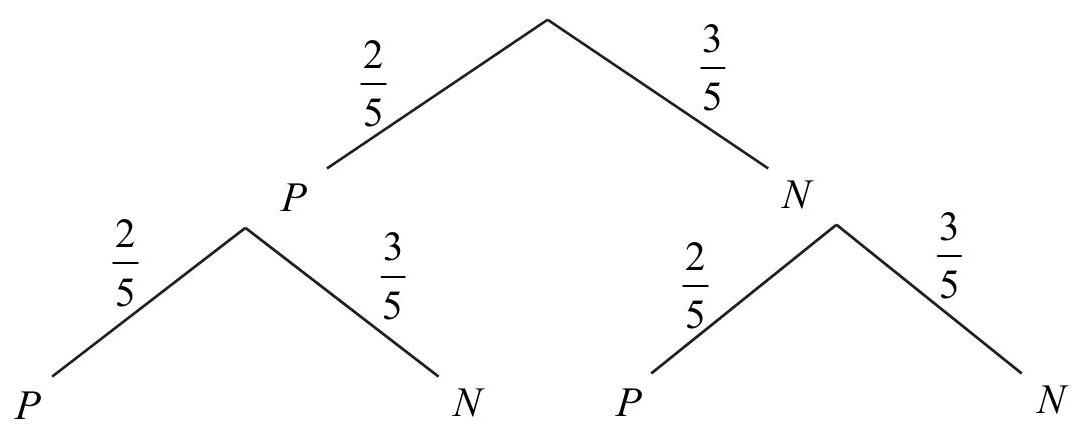
\includegraphics[max width=\textwidth, center]{2025_02_07_cbaae63d39acb23a5920g-19}

Iloczyn dwóch liczb naturalnych jest nieparzysty, jeśli obie liczby są nieparzyste. W rozważanym doświadczeniu, by zaszło interesujące nas zdarzenie, musimy wylosować dwie liczby nieparzyste. Do wyznaczenia poszukiwanego prawdopodobieństwa wystarczy zatem wymnożyć liczby z gałęzi narysowanego drzewa, odpowiadające sytuacji: $N-N$.\\
Czyli $P(A)=\frac{3}{5} \cdot \frac{3}{5}=\frac{9}{25}$.\\
IV. Użycie i tworzenie strategii.\\
7. Planimetria. Zdający korzysta z własności funkcji trygonometrycznych w łatwych obliczeniach geometrycznych, w tym ze wzoru na pole trójkąta ostrokątnego o danych dwóch bokach i kącie między nimi. (7.4).

\section*{Schemat punktowania}
\section*{Zdający otrzymuje}
gdy obliczy długość przekątnej $B D$ trapezu: $|B D|=\sqrt{68}=2 \sqrt{17}$.

\section*{Zdający otrzymuje}
gdy zapisze wysokość trapezu: $|A D|=2$ i na tym zakończy lub dalej popełni błędy.

\section*{Uwagi}
\begin{enumerate}
  \item Jeżeli zdający przy wyznaczaniu wysokości trapezu popełni błąd polegający na niepoprawnym zastosowaniu definicji funkcji trygonometrycznej lub niewłaściwym zinterpretowaniu zależności między długościami boków w trójkącie „ $30^{\circ}, 60^{\circ}, 90^{\circ}$, lub zastosowaniu niewłaściwego wzoru z sinusem kąta na pole trójkąta, to otrzymuje 0 punktów za całe rozwiązanie.
  \item Jeśli zdający przedstawi poprawny sposób obliczenia wysokości trapezu, popełni błąd przy wyznaczaniu tej wysokości, ale otrzyma jako wysokość trapezu liczbę dodatnią, to może otrzymać 1 punkt, za konsekwentne wyznaczenie długości przekątnej $B D$.
\end{enumerate}

\section*{Przykładowe rozwiązanie}
Ponieważ $|\Varangle A C D|=30^{\circ}$, więc trójkąt $A C D$ jest połową trójkąta równobocznego. Zatem

$$
|A D|=\frac{1}{2} \cdot|A C|=\frac{1}{2} \cdot 4=2 .
$$

Trójkąt $A B D$ jest prostokątny, więc możemy wykorzystać zależność z twierdzenia Pitagorasa

$$
|B D|^{2}=|A D|^{2}+|A B|^{2}
$$

Stąd otrzymujemy

$$
|B D|^{2}=2^{2}+8^{2}=68
$$

Zatem

$$
|B D|=\sqrt{68}=2 \sqrt{17} .
$$

\section*{Uwaga}
Wysokość $|A D|$ trapezu można wyznaczyć także innymi metodami.

\begin{enumerate}
  \item Z pola trójkąta $A B C$, wyznaczonego na dwa sposoby, np.: $\frac{1}{2} \cdot 8 \cdot 4 \cdot \sin 30^{\circ}=\frac{1}{2} \cdot 8 \cdot|A D|$.
  \item Z funkcji trygonometrycznej kąta w trójkącie $A C D$, np.: $\frac{|A D|}{|A C|}=\sin 30^{\circ}$.
\end{enumerate}

\section*{Zadanie 32. (0-4)}
III. Modelowanie matematyczne.\\
5. Ciągi. Zdający stosuje wzór na $n$-ty wyraz i na sumę $n$ początkowych wyrazów ciągu arytmetycznego (5.3).

\section*{Schemat punktowania}
Rozwiązanie petne

Zdający obliczy $k$ : $k=27$.

Pokonanie zasadniczych trudności zadania 3 p.\\
Zdający zapisze równanie z jedną niewiadomą $k$, które wynika ze wzoru na $k$-ty wyraz ciągu arytmetycznego: $26+(k-1) \cdot(-4)=-78$\\
i na tym zakończy lub dalej popełni błędy.

Rozwiązanie, w którym jest istotny postẹp\\
Zdający obliczy pierwszy wyraz ciągu arytmetycznego: $a_{1}=26$ i na tym zakończy lub w dalszej części rozwiązania stosuje niepoprawny wzór na wyraz $a_{k}$.

\section*{Rozwiązanie, w którym postęp jest wprawdzie niewielki, ale konieczny na drodze do pełnego rozwiązania 1 p. Zdający}
\begin{itemize}
  \item zapisze równanie $\frac{a_{1}+a_{2}+a_{3}+a_{4}+a_{5}+a_{6}}{6}=16$\\
albo
  \item wykorzysta wzór na $n$-ty wyraz ciągu arytmetycznego i zapisze wszystkie wyrazy: $a_{2}, a_{3}, a_{4}, a_{5}, a_{6}$, w zależności od $a_{1}$ i $r$ np.: $a_{2}=a_{1}+r, a_{3}=a_{1}+2 r, a_{4}=a_{1}+3 r$, $a_{5}=a_{1}+4 r, a_{6}=a_{1}+5 r$,\\
albo
  \item zapisze, że $S_{6}=6 \cdot 16$,\\
albo
  \item zastosuje wzór na sumę sześciu początkowych wyrazów ciągu arytmetycznego i wyznaczy $S_{6}$ w zależności od $a_{1}$ i $r: S_{6}=\frac{2 a_{1}+5 r}{2} \cdot 6$\\
i na tym zakończy lub dalej popełni błędy.
\end{itemize}

\section*{Uwagi}
\begin{enumerate}
  \item Jeżeli zdający realizuje strategię rozwiązania i popełnia jedynie błędy rachunkowe, to może otrzymać $\mathbf{3}$ punkty, o ile popełnione błędy nie ułatwiają rozważanego zagadnienia na żadnym etapie rozwiązania, a uzyskana liczba $k$ jest całkowita dodatnia.
  \item Jeżeli zdający popełnia błąd w interpretacji średniej arytmetycznej i poprawnie stosuje wzór na $n$-ty wyraz ciągu arytmetycznego, to może otrzymać co najwyżej 2 punkty za całe rozwiązanie.
  \item Jeżeli zdający popełnia błąd w interpretacji średniej arytmetycznej i poprawnie stosuje wzór na sumę $n$ początkowych wyrazów ciągu arytmetycznego, to może otrzymać co najwyżej 2 punkty za całe rozwiązanie.
  \item Jeżeli zdający poprawnie interpretuje średnią arytmetyczną i popełnia błąd we wzorze na $n$-ty wyraz ciągu arytmetycznego, to może otrzymać co najwyżej 2 punkty za całe rozwiązanie.
  \item Jeżeli zdający poprawnie interpretuje średnią arytmetyczną i popełnia błąd we wzorze na sumę $n$ początkowych wyrazów ciągu arytmetycznego, to może otrzymać co najwyżej 2 punkty za całe rozwiązanie.
  \item Jeżeli zdający popełnia błąd w interpretacji średniej arytmetycznej i popełnia błąd we wzorze na sumę $n$ początkowych wyrazów ciągu arytmetycznego, to może otrzymać co najwyżej 1 punkt za całe rozwiązanie.
  \item Jeżeli zdający poprawnie obliczy $a_{1}=26$, a następnie zapisze $k=27$, to otrzymuje 4 punkty.
  \item Jeżeli zdający stosuje metodę prób i błędów, sprawdzając, czy otrzymany ciąg spełnia warunki zadania (suma sześciu początkowych wyrazów jest równa 96 lub ich średnia arytmetyczna jest równa 16) i zapisze poprawny ciąg: $26,22,18,14,10,6$ oraz zapisze $a_{1}=26$ i $k=27$, to otrzymuje 4 punkty.
  \item Jeżeli zdający stosuje metodę prób i błędów, sprawdzając, czy otrzymany ciąg spełnia warunki zadania (suma sześciu początkowych wyrazów jest równa 96 lub ich średnia arytmetyczna jest równa 16) i zapisze poprawny ciąg: $26,22,18,14,10,6$ oraz zapisze $a_{1}=26$ albo $k=27$, to otrzymuje 2 punkty.
  \item Jeżeli zdający od razu zapisze poprawny ciąg: $26,22,18,14,10,6$ oraz zapisze $k=27$, ale z zapisów zdającego nie można wywnioskować, że dokonuje sprawdzenia, czy podany ciąg spełnia warunki zadania, to otrzymuje 1 punkt.
  \item Jeżeli zdający jedynie zapisze $a_{1}=26$ i $k=27$, to otrzymuje $\mathbf{0}$ punktów.
  \item Jeżeli zdający poprawnie obliczy $a_{1}$, a w drugiej części rozwiązania zapisze równanie z niewiadomą $k$ i popełni jeden błąd polegający na wpisaniu: zamiast liczby -78 liczby 78 albo zamiast liczby -4 liczby 4 , albo zamiast liczby 26 liczby -26 , to może otrzymać 1 punkt za drugi etap.
  \item Jeżeli zdający nie zapisuje, że korzysta z sumy sześciu początkowych wyrazów ciągu, a rozpoczyna rozwiązanie od zapisania zależności $\frac{a_{3}+a_{4}}{6}=16$ bez stosownych objaśnień, to może otrzymać co najwyżej $\mathbf{3}$ punkty.
\end{enumerate}

\section*{Przykładowe rozwiązanie}
Z treści zadania otrzymujemy

$$
\begin{gathered}
\frac{a_{1}+a_{2}+a_{3}+a_{4}+a_{5}+a_{6}}{6}=16, \\
\frac{a_{1}+a_{1}+(-4)+a_{1}+2 \cdot(-4)+a_{1}+3 \cdot(-4)+a_{1}+4 \cdot(-4)+a_{1}+5 \cdot(-4)}{6}=16, \\
\frac{6 a_{1}-60}{6}=16, \\
a_{1}=26 .
\end{gathered}
$$

W celu obliczenia liczby $k$ stosujemy wzór na wyraz $a_{k} \mathrm{i}$ otrzymujemy:

$$
26+(k-1) \cdot(-4)=-78, \text { a stąd } k=27 .
$$

Odpowiedź: $a_{1}=26, k=27$.

Zadanie 33. (0-4)

\begin{center}
\begin{tabular}{|l|l|}
\hline
 & \begin{tabular}{l}
8. Geometria na płaszczyźnie kartezjańskiej. Zdający wyznacza \\
równanie prostej, która jest równoległa lub prostopadła do \\
prostej danej w postaci kierunkowej i przechodzi przez dany \\
punkt (8.3). Zdający oblicza współrzędne punktu przecięcia \\
dwóch prostych (8.4). Zdający wyznacza współrzędne środka \\
odrategii. \\
odcinka (8.5). \\
\end{tabular} \\
\hline
\end{tabular}
\end{center}

\section*{Schemat punktowania}
\section*{Rozwiązanie pelne}
Zdający obliczy i zapisze wspórrzędne szukanego punktu $B$ :

$$
B=\left(\frac{102}{5},-\frac{14}{5}\right) .
$$

Pokonanie zasadniczych trudności zadania\\
Zdający:

\begin{itemize}
  \item zapisze obie równości pozwalające obliczyć współrzędne szukanego punktu $B, \mathrm{np}$.
\end{itemize}

$$
\frac{-18+x_{B}}{2}=\frac{6}{5} \mathrm{i} \frac{10+y_{B}}{2}=\frac{18}{5}
$$

albo

\begin{itemize}
  \item zapisze równanie z jedną niewiadomą, pozwalające obliczyć współrzędną szukanego punktu $B, \mathrm{np}$.
\end{itemize}

$$
\frac{\left|3 x+\frac{x}{3}-4\right|}{\sqrt{10}}=\frac{32 \sqrt{10}}{5}
$$

lub

$$
\frac{|3(12-3 y)-y|}{\sqrt{10}}=\frac{32 \sqrt{10}}{5}
$$

lub

$$
3 x-64=-\frac{1}{3}(x+18)+10
$$

i na tym zakończy lub dalej popełni błędy.\\
i na tym zakończy lub dalej popełni błędy.

\section*{Rozwiązanie, w którym jest istotny postęp}
 2 p.Zdający:

\begin{itemize}
  \item wyznaczy równanie prostej prostopadłej do prostej o równaniu $y=3 x$\\
i przechodzącej przez punkt $A=(-18,10)$
\end{itemize}

$$
y=-\frac{1}{3} x+4
$$

oraz obliczy odległość $d$ punktu $A=(-18,10)$ od prostej o równaniu $y=3 x$

$$
d=\frac{32 \sqrt{10}}{5}
$$

albo

\begin{itemize}
  \item obliczy współrzędne środka odcinka $A B: x=\frac{6}{5}$ i $y=\frac{18}{5}$,\\
albo
  \item wyznaczy równanie prostej prostopadłej do prostej o równaniu $y=3 x$\\
i przechodzącej przez punkt $A=(-18,10)$
\end{itemize}

$$
y=-\frac{1}{3} x+4
$$

oraz wyznaczy równanie prostej przechodzącej przez punkt $B$ i równoległej do symetralnej odcinka $A B$ : $y=3 x-64$\\
i na tym zakończy lub dalej popełni błędy.

\section*{Rozwiązanie, w którym postęp jest wprawdzie niewielki, ale konieczny na drodze do calkowitego rozwiązania zadania.}
\begin{itemize}
  \item wyznaczy równanie prostej prostopadłej do prostej o równaniu $y=3 x$\\
i przechodzącej przez punkt $A=(-18,10)$
\end{itemize}

$$
y=-\frac{1}{3} x+4
$$

albo

\begin{itemize}
  \item obliczy odległość $d$ punktu $A=(-18,10)$ od prostej o równaniu $y=3 x$
\end{itemize}

$$
d=\frac{32 \sqrt{10}}{5},
$$

albo

\begin{itemize}
  \item wyznaczy odległość punktu $A$ od punktu należącego do symetralnej odcinka $A B$ w zależności od jednej zmiennej, np.: $\sqrt{(x+18)^{2}+(3 x-10)^{2}}$,\\
albo
  \item wyznaczy współrzędne środka $S$ odcinka $A B$ w zależności od współrzędnych końca $B$ odcinka $A B$ : $S=\left(\frac{-18+x_{B}}{2}, \frac{10+y_{B}}{2}\right)$,\\
albo
  \item wyznaczy równanie prostej przechodzącej przez punkt $B$ i równoległej do symetralnej odcinka $A B$ : $y=3 x-64$
\end{itemize}

\section*{Uwagi}
\begin{enumerate}
  \item Jeśli zdający popełni błędy rachunkowe, które nie przekreślają poprawności rozumowania i konsekwentnie rozwiąże zadanie do końca, to może otrzymać za całe rozwiązanie co najwyżej $\mathbf{3}$ punkty.
  \item Jeżeli jedynym błędem jest:\\
a) błąd przy ustalaniu współczynnika kierunkowego prostej $A B$, to zdający może otrzymać co najwyżej 2 punkty za całe rozwiązanie;\\
b) błąd przy wyznaczaniu $b$, polegający na zamianie miejscami współrzędnych punktu $A$, to zdający może otrzymać co najwyżej 2 punkty za całe rozwiązanie;\\
c) błąd polegający na zamianie miejscami współrzędnych przy wyznaczaniu środka $S$, to zdający może otrzymać co najwyżej 2 punkty za całe rozwiązanie;\\
d) błąd polegający na błędnym podstawieniu do wzoru na odległość punktu od prostej, to zdający może otrzymać co najwyżej 2 punkty za całe rozwiązanie;\\
e) błąd polegający na zastosowaniu niepoprawnego wzoru , $\sqrt{a+b}=\sqrt{a}+\sqrt{b}$ ", to zdający może otrzymać co najwyżej 2 punkty za całe rozwiązanie.
\end{enumerate}

\section*{Przykładowe rozwiązania}
\section*{I sposób}
Wyznaczamy równanie prostej prostopadłej do prostej o równaniu $y=3 x$ i przechodzącej przez punkt $A$ :

$$
y=-\frac{1}{3} x+b .
$$

Punkt $A$ należy do prostej $y=-\frac{1}{3} x+b$, więc $10=-\frac{1}{3}(-18)+b$. Stąd $b=4$.

Obliczamy współrzędne punktu $S$ przecięcia prostej $y=3 x$ i prostej $A B$ :

$$
\left\{\begin{array}{l}
y=3 x \\
y=-\frac{1}{3} x+4
\end{array}\right.
$$

Wtedy $3 x=-\frac{1}{3} x+4$.\\
Zatem

$$
x=\frac{6}{5} \text { i } y=\frac{18}{5}, \text { czyli } S=\left(\frac{6}{5}, \frac{18}{5}\right) .
$$

Ponieważ punkt $S$ jest środkiem odcinka $A B$, więc

$$
\frac{-18+x_{B}}{2}=\frac{6}{5} \mathrm{i} \frac{10+y_{B}}{2}=\frac{18}{5} .
$$

Stąd $x_{B}=\frac{102}{5}$ i $y_{B}=-\frac{14}{5}$, czyli $B=\left(\frac{102}{5},-\frac{14}{5}\right)$.

II sposób (,„odległość punktu od prostej")\\
Równanie prostej prostopadłej do danej prostej i przechodzącej przez punkt $A$ ma postać:

$$
y=-\frac{1}{3} x+b .
$$

Wtedy $10=-\frac{1}{3}(-18)+b$, stąd $b=4$. Zatem równanie prostej $A B$ ma postać: $y=-\frac{1}{3} x+4$.\\
Punkt $B$ należy do tej prostej, więc

$$
B=\left(x,-\frac{1}{3} x+4\right) .
$$

Obliczamy odległość punktu $A$ od prostej o równaniu $y=3 x$ :

$$
\frac{|3 \cdot(-18)-1 \cdot 10|}{\sqrt{10}}=\frac{32 \sqrt{10}}{5} .
$$

Ponieważ prosta o równaniu $y=3 x$ jest symetralną odcinka $A B$, więc odległość punktu\\
$B=\left(x,-\frac{1}{3} x+4\right)$ od prostej o równaniu $y=3 x$ jest także równa $\frac{32 \sqrt{10}}{5}$.\\
Zatem otrzymujemy równanie:

$$
\frac{\left|3 x+\frac{x}{3}-4\right|}{\sqrt{10}}=\frac{32 \sqrt{10}}{5} \text {, stąd }\left|\frac{10}{3} x-4\right|=64 \text {. }
$$

Równanie to jest równoważne alternatywie równań

$$
\frac{10}{3} x-4=64 \text { lub } \frac{10}{3} x-4=-64 .
$$

Stąd

$$
x=\frac{102}{5} \text { lub } x=-18 .
$$

Obliczamy wspórtzędne punktu $B=\left(\frac{102}{5},-\frac{14}{5}\right)$.

\section*{Uwaga}
Zdający może bez wyznaczenia równania prostej $y=-\frac{1}{3} x+4$, tj. prostej prostopadłej do prostej o równaniu $y=3 x$, na której leży punkt $A=(-18,10)$, obliczyć odległość $d=\frac{32 \sqrt{10}}{5}$ punktu $A=(-18,10)$ od prostej o równaniu $y=3 x$ i zapisać równanie z jedną niewiadomą $\sqrt{(x+18)^{2}+(3 x-10)^{2}}=\frac{32 \sqrt{10}}{5}$, z którego wyznaczy pierwszą wspótrzędną środka odcinka $A B$.

\section*{III sposób}
Niech $B=(x, y)$ będzie końcem odcinka $A B$. Wtedy wspórrzędne środka $S$ tego odcinka są równe

$$
S=\left(\frac{-18+x}{2}, \frac{10+y}{2}\right) .
$$

Punkt ten leży na symetralnej odcinka $A B$, a więc na prostej o równaniu $y=3 x$, więc

$$
\begin{gathered}
\frac{10+y}{2}=3 \cdot \frac{-18+x}{2} \\
y+10=3 x-54, \\
y=3 x-64 .
\end{gathered}
$$

Prosta prostopadła do prostej o równaniu $y=3 x-64$ i przechodząca przez punkt $A$ ma równanie postaci: $y=-\frac{1}{3}(x+18)+10$.\\
Punkt $B$ należy do tej prostej, więc pozostaje rozwiązać układ równań $y=3 x-64$\\
i $y=-\frac{1}{3}(x+18)+10$. Stąd otrzymujemy

$$
\begin{gathered}
3 x-64=-\frac{1}{3}(x+18)+10, \\
3 x-74=-\frac{1}{3} x-6, \\
\frac{10}{3} x=68, \\
x_{B}=\frac{68 \cdot 3}{10}=\frac{34 \cdot 3}{5}=\frac{102}{5} .
\end{gathered}
$$

Zatem druga współrzędna punktu B jest równa $y=3 \cdot \frac{102}{5}-64=-\frac{14}{5}$, czyli $B=\left(\frac{102}{5},-\frac{14}{5}\right)$.

\section*{Uwaga}
Równanie $y=3 x-64$, które uzyskaliśmy w początkowym etapie rozwiązania to równanie prostej przechodzącej przez punkt $B$ i równoległej do symetralnej odcinka $A B$. Równanie tej prostej możemy też otrzymać, korzystając ze wzoru na odległość miedzy prostymi równoległymi oraz odległość punktu od prostej.\\
Punkt $B$ leży po przeciwnej stronie symetralnej odcinka $A B$ niż punkt $A$, na prostej $m$ równoległej do tej symetralnej, przy czym odległość prostej m od symetralnej jest równa odległości punktu $A$ od symetralnej. Prosta $m$ ma więc równanie postaci $y=3 x+c$. Ponieważ odległość między prostą $m$ i symetralną odcinka $A B$ jest równa odległości punktu $A$ od symetralnej odcinka $A B$, więc otrzymujemy równanie

$$
\frac{|c-0|}{\sqrt{10}}=\frac{|3 \cdot(-18)-10|}{\sqrt{10}},
$$

Stąd $|c|=64$, więc $c=-64$ lub $c=64$.\\
Otrzymaliśmy zatem dwie proste o równaniach $y=3 x-64$ oraz $y=3 x+64$. Drugie $z$ tych równań jest równaniem prostej przechodzącej przez punkt $A$, gdyż $3 \cdot(-18)+64=10$, więc prosta $m$ ma równanie postaci $y=3 x-64$.

Zadanie 34. (0-5)

\begin{center}
\begin{tabular}{|l|l|}
\hline
 & \begin{tabular}{l}
9. Stereometria. Zdający rozpoznaje w graniastosłupach \\
i ostrosłupach kąt między odcinkami i płaszczyznami (między \\
krawędziami i ścianami, przekątnymi i ścianami), oblicza miary \\
IV. Użycie i tworzenie \\
strategii. \\
\end{tabular} \\
\begin{tabular}{l}
tych kątów (9.2). \\
\end{tabular} &  \\
\begin{tabular}{l}
6. Trygonometria. Zdajaç wykorzystuje definicje i wyznacza \\
wartości funkcji sinus, cosinus i tangens kątów o miarach od $0^{\circ}$ \\
do $180^{\circ}(6.1)$. \\
\end{tabular} &  \\
\hline
\end{tabular}
\end{center}

\section*{Schemat oceniania}
Rozwiązanie petne 5 p.\\
Zdający obliczy cosinus kąta nachylenia krawędzi bocznej do płaszczyzny podstawy: $\frac{\sqrt{5}}{5}$.

\section*{Rozwiązanie prawie pełne}
Zdający

\begin{itemize}
  \item obliczy długość krawędzi bocznej ostrosłupa: $b=3 \sqrt{10}$\\
albo
  \item obliczy $\operatorname{tg} \alpha$\\
i na tym zakończy lub dalej popełni błędy.\\
Pokonanie zasadniczych trudności zadania\\
Zdający obliczy wysokość ściany bocznej ostrosłupa: $h_{b}=9$.\\
i na tym zakończy lub dalej popełni błędy.
\end{itemize}

Rozwiązanie, w którym jest istotny postęp\\
Zdający zapisze równanie pozwalające obliczyć wysokość ściany bocznej, np.:\\
$4 \cdot \frac{1}{2} \cdot 6 \cdot h_{b}=108$.

\section*{Rozwiązanie, w którym postęp jest niewielki, ale konieczny na drodze do pełnego rozwiązania \\
 Zdający}
\begin{itemize}
  \item zapisze zależność pomiędzy polem powierzchni bocznej a polem podstawy lub pomiędzy polem ściany bocznej a polem podstawy, np.: $P_{b}=3 P_{p}, P_{s}=\frac{3}{4} P_{p}$\\
albo
  \item zapisze dwa równania: $P_{c}=4 P_{p}$ i $P_{c}=P_{p}+P_{b}$,\\
albo
  \item obliczy pole powierzchni bocznej ostrosłupa: $P_{b}=108$,\\
albo
  \item zapisze, że $\cos \alpha=\frac{|A O|}{|A S|}$,\\
albo
  \item obliczy długość przekątnej podstawy ostrosłupa lub połowę jej długości: $|A C|=6 \sqrt{2}$ lub $|A O|=3 \sqrt{2}$.
\end{itemize}

\section*{Uwagi}
\begin{enumerate}
  \item Jeśli zdający popełni błędy rachunkowe lub przy przepisywaniu (nie dotyczy przepisywania wzorów z zestawu wzorów matematycznych), które nie przekreślają poprawności rozumowania i konsekwentnie rozwiąże zadanie do końca, to może otrzymać za całe rozwiązanie co najwyżej 4 punkty.
  \item Jeżeli jedynym błędem jest:\\
a) przyjęcie niepoprawnej zależności między polami ścian ostrosłupa: $P_{b}=4 \cdot P_{p}$, $P_{s}=4 \cdot P_{p}$,\\
b) niepoprawne zastosowanie wzoru na pole trójkąta lub niepoprawne wyznaczenie pola kwadratu, lub niepoprawne wyznaczenie długości przekątnej kwadratu, lub niepoprawne zastosowanie definicji funkcji trygonometrycznej, ale niebędące skutkiem ujawnionego błędu rachunkowego,\\
c) niepoprawne zastosowanie twierdzenia Pitagorasa,\\
d) zastosowanie niepoprawnego wzoru, $\sqrt{a+b}=\sqrt{a}+\sqrt{b}$ ",\\
e) przyjęcie obliczonej wysokości ściany bocznej jako wysokości ostrosłupa, to zdający może otrzymać co najwyżej $\mathbf{3}$ punkty za całe rozwiązanie, o ile nie popełnia innych błędów i konsekwentnie rozwiąże zadanie do końca.
  \item Jeżeli zdający popełnia jeden błąd, opisany w uwadze 2. a ponadto popełnia błędy rachunkowe, ale poprawnie realizuje strategię rozwiązania, to otrzymuje co najwyżej 2 punkty.
  \item Jeżeli zdający przyjmuje inne niż wymienione w uwadze 2a niepoprawne zależności między polami ścian ostrosłupa, to otrzymuje co najwyżej $\mathbf{1}$ punkt.
  \item Jeżeli zdający poprawnie ustala zależności między polami ścian ostrosłupa, ale przy obliczaniu wysokości ściany bocznej ostrosłupa podstawi do wzoru niepoprawną wartość za pole, to otrzymuje co najwyżej 3 punkty, o ile nie popełni innych błędów i konsekwentnie rozwiąże zadanie do końca.
  \item Jeżeli zdający przyjmuje, bez stosownych komentarzy lub obliczeń, długości odcinków w ostrosłupie, na przykład zapisuje, że wysokość ostrosłupa jest równa przekątnej podstawy lub przyjmuje, że wysokość ściany bocznej jest równa 9 , to może otrzymać za całe rozwiązanie jedynie punkty za inne części rozwiązania, np.: za wyznaczenie długości przekątnej podstawy lub za wyznaczenie cosinusa kąta.
\end{enumerate}

\section*{Przykładowe rozwiązanie}
Przyjmijmy oznaczenia jak na rysunku.\\
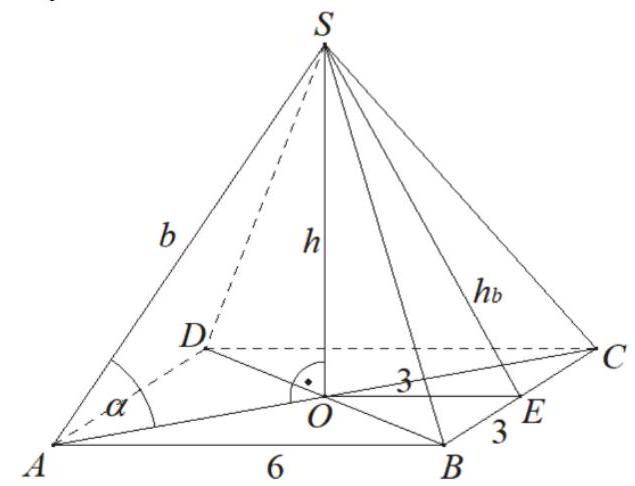
\includegraphics[max width=\textwidth, center]{2025_02_07_cbaae63d39acb23a5920g-31}

Ze wzoru na długość przekątnej kwadratu otrzymujemy

$$
|A O|=\frac{1}{2} \cdot 6 \sqrt{2}=3 \sqrt{2} .
$$

Pole podstawy ostrosłupa jest równe

$$
P_{p}=6^{2}=36 .
$$

Pole powierzchni całkowitej ostrosłupa jest 4 razy większe od pola jego podstawy, więc

$$
P_{c}=4 P_{p}=4 \cdot 36=144 .
$$

Zatem pole powierzchni bocznej ostrosłupa jest równe

$$
P_{b}=P_{c}-P_{p}=3 \cdot 36=108 .
$$

Pole powierzchni bocznej ostrosłupa jest równe

$$
P_{b}=4 \cdot P_{B C S}=4 \cdot \frac{1}{2} \cdot 6 \cdot h_{b}=12 \cdot h_{b},
$$

więc

$$
\begin{aligned}
12 \cdot h_{b} & =108, \\
h_{b} & =9 .
\end{aligned}
$$

Z twierdzenia Pitagorasa dla trójkąta $B E S$ otrzymujemy

$$
\begin{gathered}
b^{2}=3^{2}+h_{b}^{2}=9+9^{2}=9 \cdot 10, \\
b=3 \sqrt{10} .
\end{gathered}
$$

Z trójkąta $A O S$ otrzymujemy

$$
\cos \alpha=\frac{|A O|}{|A S|}=\frac{3 \sqrt{2}}{3 \sqrt{10}}=\frac{\sqrt{5}}{5} .
$$


\end{document}